%%
%% Author: Berk
%% 3/21/2019
%%

% Preamble
\documentclass[11pt]{article}

% Packages
\usepackage{amsmath}
\usepackage[margin=1in]{geometry}
\usepackage{amsmath,amsthm,amssymb}
\usepackage{comment}
\usepackage[acronyms]{glossaries}
\usepackage{graphicx}
\usepackage{tikz}
\usepackage{tikz-3dplot}
\usetikzlibrary{shapes.geometric}

\newacronym{sdp}{SDP}{semidefinite program}
\newacronym{ceg}{CEG}{Convex Engineering Group}
\newacronym{gp}{GP}{Geometric Program}
\newacronym{mc}{MC}{Monte Carlo}
\newacronym{sp}{SP}{Signomial Program}
\newacronym{rgp}{RGP}{Robust Geometric Program}
\newacronym{rsp}{RSP}{Robust Signomial Program}
\newacronym{ro}{RO}{Robust Optimization}
\newacronym{so}{SO}{Stochastic Optimization}
\newacronym{mdo}{MDO}{Multidisciplinary Design Optimization}
\newacronym{dc}{DC}{difference-of-convex}
\newacronym{nlp}{NLP}{Nonlinear Program}
\newacronym{rhs}{RHS}{right hand side}
\newacronym{lhs}{LHS}{left hand side}
\newacronym{cv}{CV}{coefficient of variation}
\newacronym{srm}{SRM}{solid rocket motor}

\makeglossaries

% Document
\begin{document}

    \title{SDP relaxations for solid rocket motor shape optimization}
    \author{Berk Ozturk}
    \maketitle

    \section{Introduction}
    
    Shape optimization is inherently an infinite-dimensional problem,
for which tractable formulations are of particular interest.
    It appears in a range of problems in aerospace design, and most notably
    aerostructural optimization which has been the bread-and-butter of the \gls{mdo} field.

	These is very little literature, if any, on solid rocket conceptual design,
for several reasons. (1) The physics governing internal reactive flow is extremely complex,
and there are no open-source tools that don't require domain knowledge and
can efficiently simulate such a scenario.
(2) There are few entities that design and build solid rocket motors, and since they have
large amounts of resources and time and little competition there has been no impetus
improve solid rocket design methods. (3) Solid rocket motors are relatively limited
in capability because their burn rate is almost completely uncontrollable other
than by properly designing the internal geometry of the rocket or actuating the
throat of the nozzle. For this reason liquid propellant rockets have been preferred for
many applications. (4) Rocket design is often proprietary due to arms regulations.

This is an interesting problem where a \gls{sdp} for geometry design,
    coupled with first-order flow models may offer a good alternative to
    more traditional gradient-based methods which are used alongside
    high-fidelity internal flow simulations.
    Furthermore, problems of the form I will pose appear in other interesting
    aerospace problems, such as hypersonic vehicle external geometry design,
    so the formulation has valuable extensions.

    \section{Brief background on solid rocket motors}

A \gls{srm} is extremely simple. Think a candle with a casing on it to contain the pressure and hot gas from burning material,
and a nozzle at the end to make the high-pressure flow go supersonic and generate thrust.
There are a few differences between \gls{srm}s and candles.
First is the fact that solid rocket motor fuel contains propellant and oxidizer (wax and oxygen),
whereas a candle only contains fuel and relies on an external source of oxygen (eg. the air around it).
As a result, \gls{srm}s can even be lit underwater or in a vacuum;
they are extremely robust. The second difference is the geometry.
A candle is akin to an end-burning rocket; the wax only burns at the candle's melty end.
A \gls{srm} usually has some geometry down the bore of the rocket which runs all the way down its length for greater surface area.
(An end-burning rocket is almost completely uninteresting since there is not a significant aspect of geometry to design.)
The third is the presence of the nozzle. Without it, the flow would stay sonic when exiting the bore and
not generate thrust effectively. The disadvantage of solid rocket motors is that
they are essentially a runaway chemical reaction, an explosive that is confined in a casing,
whose rate is controlled by the area of the throat of the nozzle.
Once lit, they cannot be stopped or controlled, like liquid rockets or jet engines
can be by modulating the amount of propellant and oxidizer.
Therefore the design of the geometric pattern in a \gls{srm}'s bore is critical for a proper burn rate.


    \section{Approach}
    
    I am developing a two-stage approach to the \gls{srm} design problem.
    The first stage is a 1D quasi-steady rocket optimization model,
    which determines both the internal flow quantities and a basic description
    of the internal geometry. I have already developed this model,
    which takes the following inputs:
    \begin{itemize}
    \item Coarse time and spatial discretization of the rocket sections
    \item The desired thrust profile of the rocket
    \item Bounds on the rocket external dimensions, if desired
    \item Material properties of the propellant  
    \end{itemize}
    
\tdplotsetmaincoords{50}{130}
\tdplotsetrotatedcoords{0}{90}{0}

\begin{figure}
\begin{center}
\begin{tikzpicture}[tdplot_main_coords]
    \draw[thick,->] (0,0,0) -- (1,0,0) node[anchor=north east]{$l$};
    \draw[thick,->] (0,0,0) -- (0,-1,0) node[anchor=south west]{$r$};
    \draw[thick,dashed] (0,0,0) -- (-4,0,0) node[anchor=north west]{$$};
    % Blue circles
    \tdplotdrawarc[tdplot_rotated_coords, color=blue]{(0,0,-4)}{2}{0}{360}{anchor=south west}{$\pi r^2$};
    \tdplotdrawarc[tdplot_rotated_coords, color=blue]{(0,0,0)}{2}{0}{360}{anchor=south west}{$$};
    % Blue dashed lines
    \draw[thick,dashed,color=blue] (0,-1.414,1.414) -- (-4,-1.414,1.414) node[anchor=south east]{$l_{\rm{sec}}$};
    \draw[thick,dashed,color=blue] (0,1.414,-1.414) -- (-4,1.414,-1.414) node[anchor=north west]{$l_{\rm{sec}}$};

    % Tophalf, top circle
    \tdplotdrawarc[tdplot_rotated_coords, color=red]{(-0.25,0.25,-4)}{1}{25}{248}{anchor=north west}{$$};
    % Top half, bottom circle
    \tdplotdrawarc[tdplot_rotated_coords, color=red]{(0.25,-0.25,-4)}{1}{205}{428}{anchor=north west, right=0.5cm, above=0.5cm}{$A_{in}$};
    % Bottom half, top circle
    \tdplotdrawarc[tdplot_rotated_coords, color=red]{(-0.25,0.25,0)}{1.25}{28}{243}{anchor=north west}{$$};
    % Bottom half, bottom circle
    \tdplotdrawarc[tdplot_rotated_coords, color=red]{(0.25,-0.25,0)}{1.25}{208}{425}{anchor=north west, right=0.5cm}{$A_{out}$};

    % Red dashed lines
    \draw[thick,dashed,color=red] (0,-0.85,0.85) -- (-4,-0.67,0.67) node[anchor=south east]{$$};
    \draw[thick,dashed,color=red] (0,0.85,-0.85) -- (-4,0.67,-0.67) node[anchor=north west]{$$};
\end{tikzpicture}
\end{center}
    \caption{Labeling of a single section of the rocket. }
    \label{fig:SRMsection}
\end{figure}

The optimization model, which is a signomial program, determines the
flow properties inside and thrust generated by a rocket that has
been partitioned into $n_x$ of sections that evolve in $n_t$ timesteps.
    Figure~\ref{fig:SRMsection} shows a potential cross-section of such a \gls{srm}.
The physical model assumes quasi-steady flow during each timestep, where the fluid travels strictly
in the $l$ direction down the bore drawn in red, and the conservation laws are enforced at
each bore cross-sectional area $A$. The output variables of this model are:
    \begin{itemize}
    \item The material properties of the fuel burned in a given section in one timestep, which are:
        \begin{itemize}
        \item Porosity of fuel
        \item Mass fraction of propellant
        \item Mass fraction of accelerant
        \item Mass fraction of filler
        \end{itemize}
    \item The arc lengths of shapes of $A_{in}$ and $A_{out}$
    \item The cross-sectional areas of $A_{in}$ and $A_{out}$
    \end{itemize}
    
The idea is to take these output variables, and map them onto a series of 
non-intersecting univariate polynomials $p(\theta, t_i), t_i = [1,2,...,n_t]$ which describe the internal geometry of the rocket. Or potentially, they could be mapped to the bivariate polynomial $p(\theta,t)$ which has the requirement to be monotonically increasing in $t$ (equivalent constraint to having non-intersecting polynomials $p(\theta, t_i)$). To give context about the kinds of cross-sectional shapes that are currently used in rocket design, see Figure~\ref{fig:potentialShapes}. The sky really is the limit. The hope is that this problem has a \gls{sdp} relaxation that can find polynomials that can fulfill the constraints, at a minimum in a least-squares sense, since feasibility is not guaranteed. 

\begin{figure}
\begin{center}
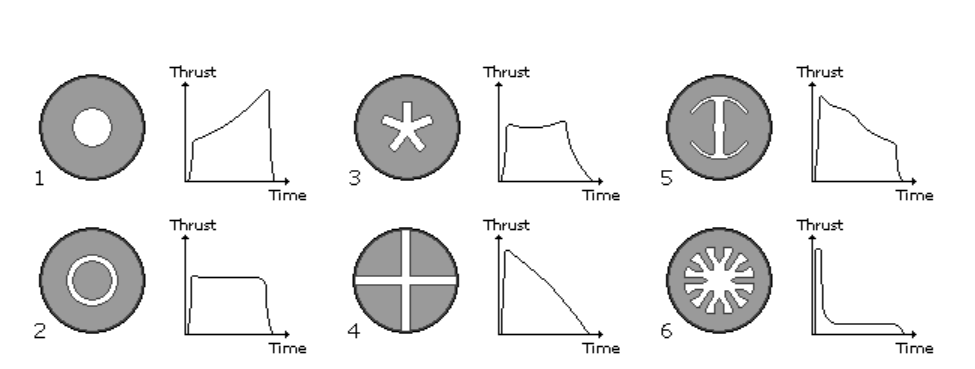
\includegraphics[width=0.7\linewidth]{figures/potentialShapes.png}
\label{fig:potentialShapes}
\caption{Different thrust profiles may result in very different potential internal configurations of the rocket. Image courtesy of Robert A. Braeunig.}
\end{center}
\end{figure}

\section{Constraints}

I want to elaborate more on the constraints of the problem, and how one might go about formulating a \gls{sdp}. These are imposed at $n_x+1$ cross-sections to determine the polynomials describing the internal geometry at different cross-sectional slices of the rocket. The surface geometry in between the sections will be described through interpolation. 

\begin{itemize}
\item \textbf{The integral difference between the cross-sectional areas of the shape must be equal to the fuel burnt in a given time step, as determined by the first-stage problem.} In other words: 
\begin{equation}
\int\limits_{-\pi}^{\pi} p(\theta, t_i) + \Delta A_{p, t_i} = \int\limits_{-\pi}^{\pi} p(\theta, t_{i-1})
\end{equation} We can determine this easily through Gaussian quadrature, which makes this a linear constraint on the coefficients of the polynomial $p(\theta, t_i)$. 
\item \textbf{The arc length of the polynomial must be equal to the arc length $l_b$ as determined by the first-stage problem.} This seems like a pretty complex constraint to figure out how to do, since the arc length of an arbitrary polynomial curve has no closed-form solution. In $\theta$, it can be represented as:
\begin{equation}
s(t_i) = \int\limits_{-\pi}^{\pi} \sqrt{r^2 + \Big(\frac{dr}{d\theta}\Big)^2} d\theta, ~r = p(\theta, t_i)
\end{equation}
Perhaps this can be approximated using a triangle approximation:
\begin{equation}
s(t_i) \approx \sum\limits_i r_{i}r_{i-1}\rm{sin}(\delta\theta)
\end{equation}
Clearly this approximation is best when the difference $r_{i} - r_{i-1}$ is small. The relaxation of this constraint is a quadratic constraint on the coefficients of $p$, for a know $\delta\theta$. 

\item \textbf{The shapes must never intersect.} Since the flame front must strictly regress as a result of burning, the polynomials describing the shapes must have no common roots. This is a sum-of-squares constraint on the difference of the univariate polynomials $p(\theta, t_i)$, or a constraint for bivariate polynomial $p(\theta, t)$ to be monotonically increasing in $t$.
\item\textbf{The shapes must not intersect the unit circle.} Since fuel can only be contained inside the casing of the rocket, we set an upper bound on the polynomials. This can be achieved by making sure the polynomials don't have common roots with the constant polynomial representing unit circle. This will also require that the negative of the polynomials be a sum-of-squares. 
\item \textbf{Regularity conditions on the shape of the polynomials.} Not sure what form these will take, but the shapes of the polynomials must `follow' each other. Furthermore, it would be nice if the polynomial was continuous in its second-derivative since it has a periodic boundary condition on the circle. These would all be constraints on $\frac{dp}{d\theta}$ and $\frac{d^2p}{d\theta^2}$, which are polynomials of degree $d-1$ and $d-2$ since we are discussing univariate or bivariate polynomials. 
\end{itemize}

\section{Conclusion}

I think that shape optimization presents exciting frontiers for the use of \gls{sdp}s in engineering.
    6.256 has been quite theoretical so far, so I am excited to take these real-world constraints and
    try to formulate a tractable approximation of the second-stage \gls{srm} optimization problem.
    I will be bothering you a lot in the weeks following Spring Break to try and get your insight and figure
    out if I am on the right track. Thanks!

\end{document}
